\chapter{Software Development Method}\label{chap:sw_dev_method}
One of the great challenges this semester is to coordinate the development process across all 14 groups. To ensure a smooth process we define the development method of the multi-project.

%\todo{Ulrik recommends: A chapter describing the role of this project in the setting of the multi-project. This includes ``an analysis of an organizational context''.}

\begin{chapterorganization}
  \item in \sectionref{sec:project_overview} we describe how the multi-project is organized and introduce the hierarchy in the project;
  \item in \sectionref{sec:swmethod_ourgroup} we describe the software development method in our group;
  \item in \sectionref{sec:multi_project_group_roles} we detail the responsibilities delegated to most groups.
\end{chapterorganization}

\begin{abbreviations}
  \item[\gui] Graphical User Interface
  \item[\db] Database
  \item[\bd] Build \& Deployment
  \item[PO] Product Owner
\end{abbreviations}

\section{Multi-Project Organization Method}\label{sec:project_overview}
The multi-project consists of 14 groups. Two groups of two and the remaining groups consists of four people each.  All groups collaborate on building the Giraf applications. The groups are organized into three subprojects: \emph{Graphical User Interface} (\gui), \emph{databases} (\db), and \emph{build and deployment} (\bd) by recommendation of the semester coordinator.

The \gui groups deal with bugs and implementing new features in the front-end apps. The \db groups manage and maintain the database. The \bd groups control the tools supporting the building and testing environment as well as the deployment of the apps.

The multi-project groups work with an iterative development method, and the semester is divided into four iterations. No groups have any prior experience with the code base at the start of the project and previous developers indicated uncertainties with the users' requirements\kimnote{Hvis i har en kilde på det her så indsæt den gerne :)}. This makes an agile method suited for the project. Suppose the multi-project is organized in a traditional method. Then the multi-project groups will spend much time initially analyzing the current code base and future requirements, rather than actually work on making the code base work (a prime wish for the external customer). These requirements may change over time, which makes it difficult to deliver what the users want.

The agile method used for the project is Scrum, and the groups are organized as Scrum of Scrums\todo{Uddyb eventuelt}\kimnote{Det er nok med en kilde på hvad i mener når i skriver scrum og scrum. Hvis i afviger fra jeres kilde så skal i forklarer hvad i gør anderledes og hvorfor!}. \figureref{fig:multi_project_organization} shows the structure of the multi-project organization, which consists of three levels:

\begin{description}
  \item[Multi-Project Level] The purpose of the overall level is to ensure that the roles, work products, and meetings are followed as intended. That is, that the development method is followed. A weekly meeting is held where the product backlog is maintained, the status of each subproject is discussed, and the development method and roles are evaluated. Every group has at least one representative at the weekly multi-project meetings.
  \item[Subproject Level] Each subproject has the responsibility of solving a number of user stories related to either \gui, \db, or \bd. This level follows Scrum of Scrums. Representatives from each group in a subproject have sprint planning and sprint end meetings with the other members of the subproject and hold at minimum two Scrum meetings a week. We chose not to meet every day because we think that it will steal to much time, compared to the benefits. 
  \item[Group Level] Each group solve some of the user stories of their subprojects. While Scrum of Scrums dictates that Scrum is followed at all levels, this is not the case for this multi-project organization. This is of course a major deviation from Scrum of Scrums. When initially deciding the software development method, some groups expressed an interest in not running Scrum. Thus, each group is given the freedom to organize how they see fit. However, all groups are expected to fill in the work products and attend the meetings described later.
\end{description}

\fig{multi_project_organization}{Illustration of multi-project organization}{Illustration of multi-project organization. \todo{Temporary figure. Make a nicer in tikz and add some more description.}\kimnote{jeg kan gode lide at i markere "groups" det kunne i også gøre med "teams/subprojects"}}

\subsection{Work Products}
Two work products from Scrum are used, every group is expected to produce these artifacts:

\begin{description}
  \item[Product Backlog] The product backlog contains the user stories that the customers specify. These user stories are the requirements for the product from a user perspective \parencite{larman2003}. On the multi-project level, there is a a product backlog that contains all the user stories for the entire multi-project is used. The purpose of the multi-project level is to maintain the product backlog for the entire multi-project. The user stories in the product backlog are categorized according to each subproject. This enables each subproject to manage their user stories themselves, removing unnecessary management from the multi-project level.
  \item[Release Backlog] The release backlog contains the user stories that must be finished by the end of the current sprint \parencite{larman2003}. These user stories are decided on sprint planning meetings that each subproject hold.\kimnote{so the Release backlog contains all stories for the subproject? please elaborate! :)}
\end{description}

Since it is not required for each group to use Scrum at the group level, there is no sprint backlog (collection of tasks) shared among all groups.

\subsection{Roles}
Two roles from Scrum are used in the multi-project:

\begin{description}
  \item[Scrum Master] On the multi-project level, we are responsible for the development method. This means that we act as Scrum masters on the multi-project level. On the subproject level, one person is charge of the meetings --- they make sure that the Scrum meetings on this level are held. On the group level, each group is free to do what they see fit.
  \item[Product Owner] The product owner (PO) is responsible for maintaining contact with the customers and being their representatives. It can be difficult to have a single PO with an external customer as customer in the multi-project. Therefore, the \bd and \db groups often do not have the external customer as their direct customer. Rather, these groups help the \gui groups achieve their goal by building solutions for them. The external customer is often not interested in the implementation details of build and database interfaces.

As such, we decided during sprint 1 that there are three POs in the multi-project, one for each subproject. The customer for the \gui PO is the external customer, whereas the customers for the \db and \bd POs are the groups of the other subprojects, as illustrated in \figureref{fig:po_illu}.

\end{description}

\begin{figure}%
\centering
\tikzsetnextfilename{po_illustration}
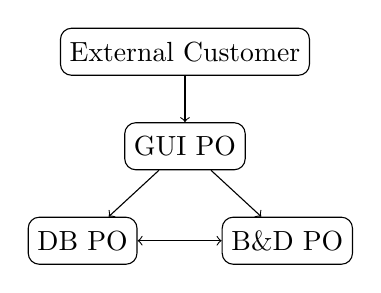
\begin{tikzpicture}[
  simple/.style={draw, rounded corners, minimum height=1.7em}]
  \node[simple] (extcust) at (0,1.2) {External Customer};
  \node[simple] (guipo) at (0,0) {GUI PO};
  \node[simple] (dbpo) at (-1.3,-1.2) {DB PO};
  \node[simple] (bdpo) at (1.3,-1.2) {B\&D PO};
  
  \draw[->] (guipo) to (dbpo);
  \draw[->] (guipo) to (bdpo);
  \draw[<->] (dbpo) to (bdpo);
  \draw[->] (extcust) to (guipo);
  
\end{tikzpicture}
\caption{Illustration of product owners}%
\label{po_illu}%
\end{figure}

%\fig{po_illu}{Illustration of product owners}{Illustration of product owners. \todo{Temporary figure. Make a nicer in tikz and add some more description. In particular of the arrows.}}

\subsection{Meetings}\label{sec:meetings}
Each week there is a meeting at the multi-project level. At this meeting the status of the groups in the multi-project is presented and the development method is evaluated. This ensures that all groups know the current status of the project, and that the development method can be continually improved.

At the subproject level, a Scrum meeting is held at least two times a week. It is up to each subproject to organize these meetings. In addition to the Scrum meeting at the subproject level, each group is advised to follow Scrum internally\kimnote{reformulate}.

Since there are three product owners in the entire multi-project, three sprint ends and sprint planning meetings are held after and before each sprint\kimnote{reformulate}. These meetings were proposed by us, following the recommendation from \textcite{bird_davies_2007}, and afterwards approved by the other groups.

\begin{description}
  \item[Sprint Planning Meetings]
  The purpose of the sprint planning meetings is to ensure that the product backlog is up to date and to select user stories for the release backlog.
  \begin{description}
    \item[GUI] At this sprint planning only one representative from each GUI group participate as \emph{pigs} (people who are allowed to talk), as well as the GUI PO and one representative from the other PO groups (although they have a less important role at this meeting). All other people in the multi-project are \emph{chickens} (people who are not allowed to talk). This meeting is held with the external customers. By making it so that primarily the \gui groups are pigs, the external customers are abstracted from internal development such as continuous integration and database management.
    \item[\db and \bd] There are separate sprint planning meetings for \db and \bd, where each subproject establishes the needs of the other subprojects. These meetings are internal, and the external customers do not participate, since \db and \bd do not have these as direct customers. \db and \bd will primarily have the GUI groups as their customers, who need various services from the \db and \bd subprojects, in order for them to fulfill their own user stories directly related to the external customers. However, it might be that \db needs something from \bd and vice versa. Again, this abstracts the external customers from internal development.
  \end{description}
  \item[Sprint End Meetings]
  At the sprint end meetings, the work done in the sprint is presented to the customers.
  \begin{description}
    \item[GUI] At this meeting the external customers are presented with the work of the GUI groups. Only the GUI groups participate as pigs at this meeting.
    \item[\db and \bd] \db and \bd hold each \kimnote{each hold} a separate sprint end meeting where they show the groups in the other subprojects what they have done in a sprint. The external customers are not present at these meetings, so that they are not bored with internal details.
  \end{description}
\end{description}

\subsection{Office Hours}
A vital part of working agile involves being able to easily communicate with all members of the team\kimnote{You did not define what a team is, I guess you meant the multi-project members}. To ensure this all groups must be reachable on mail all weekdays 09:00--15:00, and preferably be in the group rooms. An exception for this is when there are courses.

\subsection{Tools}\label{sec:tools}
To support the development method of the multi-project, an online project management tool, Redmine\kimnote{Cite or footnote}, is used. This tool was in use the previous year, and so this year continues to use it. The main features are:

\begin{description}
  \item[Wiki] A wiki is used for various information, such as guides, how the development method is structured, meeting summaries, etc. Previous years had several separate wikis for each subproject. This year there is a single wiki providing central information.
  \item[Forum] The forum is used for non-crucial communication. It is mostly used for non-work related discussions such as social events. Groups are encouraged to communicate to each other directly by going to each other's group rooms, rather than using the forum.
  \item[Issue Tracker] The issue tracker is not used as a traditional issue tracker, but instead customized to so that it contains the product backlog and release backlog\kimnote{consider calling it what it is!}. The user stories are mixed in with tasks, support issues, meetings, and other items. Filters can be used to isolate specific items, such as user stories in the product backlog. This setup is not ideal as it can be hard to manage at times, but it is what the multi-project has available without much more needed effort. We collaborated with \group{3} (Redmine general) and \group{10} (user story and task trackers) to set this up\kimnote{who designed this setup? if you did then say it! What was your role in this collaboration?}\kimnote{I think this "collobration" should be a part of sprint 1, again, I will elaborate on this at our meeting.}.
\end{description}

Redmine also contains other features such as a roadmap, burndown charts, and news. While these features are present on the main page, they are not used. The burndown chart in particularly is not used since no common sprint backlog is used, and as such the burndown chart cannot be used at the multi-project level.

Also, a Gantt chart feature had been installed by previous years. The Scrum method does not advocate Gantt charts or other dependency charts \parencite{larman2003}. As such, we collaborated with \group{3} to remove this from Redmine. The other unused features have not been removed, since it was deemed unnecessary to spend time on doing so. \kimnote{Same as above, work you do in a sprint should be describe in a sprint.}

\section{Software Development Method in Our Group}\label{sec:swmethod_ourgroup}
As all groups are recommended to follow the Scrum development method, our group follows it. With it we hold a Daily Scrum each morning where we summarize our work since last time and what we intent to do until the next Daily Scrum \todo{Er dette ikke unødvendigt at nævne? Vi kører jo Scrum, så selvfølgelig har vi et Daily Scrum}.\kimnote{I think it is fine to briefly mention what parts of scrum you do use.}

In addition to the previously described work products, we use a sprint backlog. After a sprint planning where user stories have been assigned to each group, we then split the user stories assigned to us into tasks and estimate those tasks using planning poker. Our unit of estimation is in half days, with the smallest unit being 1. This means that tasks that can actually be completed in less than a half day, may become overestimated. However, since there is an inherent imprecision in our estimations, this is not an issue. Our sprint backlog is physically placed on a wall, so that we can easily manage our tasks. In addition to the sprint backlog we use a burndown chart to measure our progress.

We also initially used Redmine as our Scrum board, but due to Redmine being very slow and tedious to update, we replaced it with a physical Scrum board. As not all groups do Scrum and thus estimate tasks, this decision has no impact on the performance of the multi-project. \todo{Should we delete or move this paragraph?}

\section{Group Roles in Multi-Project}\label{sec:multi_project_group_roles}
The multi-project contains responsibilities that have been assigned to the groups within the multi-project. These roles include management of Redmine, server, Git, Jenkins and other various tasks. Following they are shortly described:

\begin{description}
  \item[Redmine --- General] Maintaining users, roles, and plugins on Redmine as well as managing work across the other Redmine groups below.
  \item[Redmine --- Wiki] Structuring and maintaining the wiki. They also read the content and make sure it is adequate, and notify the relevant groups if problems are found.
  \item[Redmine --- Forum] Structuring and moderating the forum.
  \item[Redmine --- User Story and Task Tracking] Structuring and maintaining the user story and task tracker as well as helping people creating the items in the tracker. They also maintain guidelines for task creation.
  \item[Server] Maintaining the server software and controlling access to the server. They install and upgrade software upon request and help solving issues requiring root access.
  \item[Git] Maintaining the Git repositories and controlling access to these. Furthermore, they issue guidelines for Git usage.
  \item[Jenkins] Maintaining the Jenkins setup. This is the responsibility of our group, and as such will be detailed in this report.
  \item[Process] Supervising, developing, and refining the process method. This is also the responsibility of our group, and will as such also be detailed in this report.
  \item[Code Style] Developing and encouraging a code style across all code.
  \item[Customer Relations] Maintains customer relations. They review and send any email sent to the external customers.\todo{Dette ændrer sig måske i et senere sprint}
  \item[Web Administrator] Maintains the public project website \url{http://giraf.cs.aau.dk}.
  \item[Android Guru] Persons with experience developing Android apps, and who can be asked for help.
  \item[Google Analytics and Google Play] Maintaining the Google Play listing of the software and generating guidelines for how to get crash reports from Google Analystics. Furthermore, they published the builds during the first sprints. \todo{Specify this later}.
  \item[Graphics] Developing a graphical style and enforcing this as well as creating the graphics upon request.
\end{description}

\todo{Skriv i parentes eller noget hvilke grupper der har hvilke roller} \todo{(Michael): Det kan ændre sig. Måske kan det ikke gøres?}
